\chapter{DESAIN DAN PERANCANGAN}
    Pada bab ini dibahas mengenai analisis dan perancangan sistem.
    
    \section{Deskripsi Umum Sistem}
    	\indent Sistem yang akan dibangun pada tugas akhir ini adalah sebuah sistem yang dapat melakukan automasi uji beban terhadap suatu web. Uji beban pada sistem akan berjalan secara headless menggunakan sebuah tester yaitu Headless Chrome. Headless Chrome akan mendapatkan data uji beban ketika mengakses web yang diuji, sedangkan yang digunakan untuk mengambil data uji beban adalah sebuah pustaka Node yaitu Puppeteer. Sistem juga akan menggunakan Docker sebagai infrastruktur, sehingga Docker dapat digunakan sebagai load generator untuk melakukan uji beban yang bisa disebut kontainer.
    	
    	\indent Kontainer yang akan dipasang pada sistem membutuhkan sebuah alat orkestrasi untuk memanajemen kontainer secara otomatis, alat orkestrasi yang digunakan adalah Docker Swarm. Docker Swarm akan melibatkan 3 node host yang akan dibagi menjadi 1 node host sebagai swarm manager dan 2 node host sebagai worker. Docker Swarm akan bertanggung jawab dalam mendistribusikan kontainer ke masing-masing swarm node yang tergabung pada lingkungan swawrm atau bisa disebut sebagai load balancer.
    	
    	\indent Proses uji beban akan diproses user melakukan request skenario uji beban pada web service yang disediakan sistem. Kemudian controller pada web service akan mengirimkan skenario uji pada kontainer terpilih untuk melakukan pengujian. Setiap kontainer akan terinstall Headless Chrome dan Puppeteer. Headless Chrome akan mendapatkan data uji beban dan automasi pengambilan data uji beban dilakukan oleh Puppeteer. Puppeteer akan melakukan ekstraksi data uji beban menjadi satuan millisecond(ms). 
    	
    	\indent Sistem akan menyediakan basis data untuk menyimpan data yang diperlukan sistem. Basis data akan dipasang diluar lingkungan swarm dan lingkungan web service. Sistem juga menyediakan antarmuka pengguna berupa web yang akan digunakan untuk melihat laporan hasil uji beban. Sedangkan untuk mengatasi multiuser sistem akan menggunakan Task Scheduler atau Queue(antrian).
    
    \section{Kasus Penggunaan}
	    \begin{figure}[H]
	    	\centering
	    	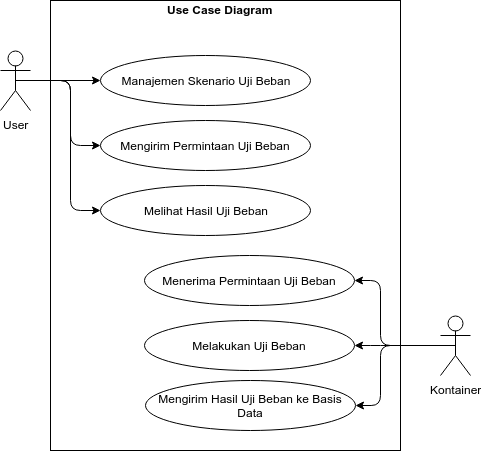
\includegraphics[width=9cm,height=9cm]{Images/C-3/usecasediagram.png}
	    	\caption{Diagram kasus penggunaan}
	    	\label{usecased}
	    \end{figure}
    	Terdapat dua aktor dalam sistem yang akan dibuat yaitu User dan Kontainer. User merupakan aktor yang bisa melakukan manajemen pada skenario yang ingin diuji dan melihat hasilnya, sedangkan Kontainer merupakan aktor yang akan digunakan sebagai load generator untu melakukan uji beban. Diagram kasus penggunaan digambarkan pada Gambar \ref{usecased} dan dijelaskan masing-masing pada Table \ref{tabelusecase}.
    	
    	\begin{longtable}{|p{0.20\textwidth}|p{0.30\textwidth}|p{0.35\textwidth}|}
    		\caption{Daftar kode kasus penggunaan} \label{tabelusecase} \\
    		\hline
    		\textbf{Kode Kasus Penggunaan} & \textbf{Nama Kasus Penggunaan} & \textbf{Keterangan} \\ \hline
    		\endhead
    		\endfoot
    		\endlastfoot
    		UC-0001 & Manajemen Skenario Uji Beban & User dapat menambah, melihat dan menghapus skenario uji beban \\ \hline
    		UC-0002 & Mengirim Permintaan Uji Beban & User dapat mengirimkan permintaan uji beban ke sistem melalui web service yang disediakan \\ \hline
    		UC-0003 & Melihat Hasil Uji Beban & Ketika proses uji beban selesai, user dapat melihat hasilnya di antarmuka pengguna web service yang disediakan \\ \hline
    		UC-0004 & Menerima Permintaan Uji Beban & Proses dimana kontainer akan menerima permintaan uji beban dari User \\ \hline
    		UC-0005 & Melakukan Uji Beban & Proses dimana kontainer akan melakukan uji beban sesuai skenario yang dikirim \\ \hline
    		UC-0006 & Mengirim Hasil Uji Beban ke Basis Data & Ketika kontainer telah selesai melakukan pengujian, data yang didapatkan akan dikirim ke basis data MySQL \\ \hline
    	\end{longtable}
    
    \section{Arsitektur Sistem}
	    \begin{figure}[H]
	    	\centering
	    	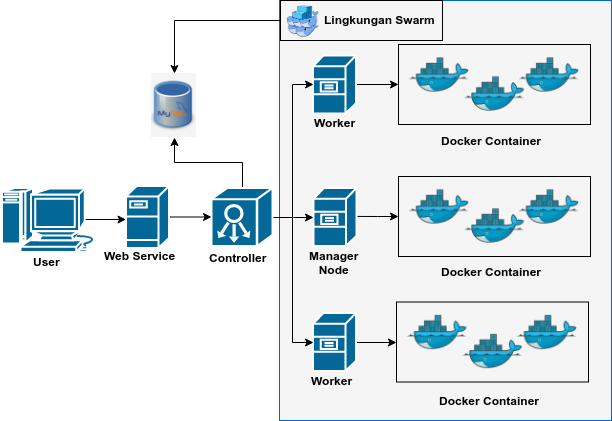
\includegraphics[width=10cm,height=6cm]{Images/C-3/arsitektursistem.png}
	    	\caption{Desain arsitektur sistem}
	    	\label{arsitekturumum}
	    \end{figure}
    	
    	\indent Pada sub-bab ini, akan dibahas mengenai tahap analisis arsitektur, analisis teknologi dan desain sistem yang akan dibangun. Arsitektur sistem secara umum ditunjukkan pada Gambar \ref{arsitekturumum}.

    	\subsection{Desain Umum Sistem}
    		Berdasarkan yang dijelaskan pada deskripsi umum sistem, dapat diperoleh beberapa kebutuhan sistem antara lain:
    		\begin{enumerate}
    			\item Load generator untuk melakukan uji beban.
    			\item Tester yang bisa mengambil data uji beban.
    			\item Web service sebagai antarmuka pengguna.
    			\item Basis data untuk menyimpan data sistem.
    			\item Task Queue untuk menangani kasus request lebih dari satu user.
    		\end{enumerate}
    	
    		Untuk memenuhi kebutuhan sistem yang dijelaskan sebelumnya, penulis membagi menjadi beberapa komponen sistem yang akan digunakan pada tugas akhir ini.
    		
    		\begin{enumerate}
    			\item Load generator \\
    				Berfungsi sebagai pengganti user yang akan melakukan akses web melalui browser.
    			\item Pengambil data uji beban \\
    				Berfungsi untuk mengambil data uji beban ketika load generator mengakses web dari browser.
    			\item Service Controller \\
    				Berfungsi sebagai pengatur sistem uji beban yang terdiri :
    				\begin{itemize}
    					\item Web Service \\
    						Berfungsi sebagai tampilan antarmuka pengguna untuk menggunakan sistem.
    					\item Basis Data \\
    						Berfungsi untuk menyimpan data yang digunakan untuk menyimpan segala data yang dibutuhkan oleh sistem.
    					\item Task Queue \\
    						Berfungsi untuk membuat task scheduler atau antrian untuk menangani kasus request lebih dari satu user.
    				\end{itemize}
    		\end{enumerate}
    	
    	\subsection{Perancangan Load Generator}
	    	\begin{figure}[h]
	    		\centering
	    		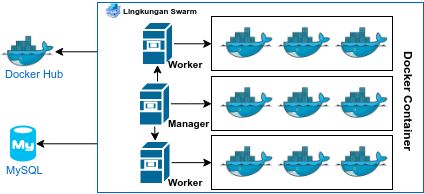
\includegraphics[width=11cm,height=6cm]{Images/C-3/dockerdesain.png}
	    		\caption{Desain perancangan load generator}
	    		\label{dockerdesain}
	    	\end{figure}
    		Komponen load generator akan difungsikan sebagai pengganti pengguna yang mengakses ke suatu web melalui browser. Komponen yang akan digunakan sebagai load generator adalah Docker atau bisa disebut kontainer. Ketika melakukan pemasangan kontainer sebuah Docker Image, untuk memenuhi hal tersebut, pada tugas akhir ini penulis akan membuat sebuah Docker Image yang akan diunggah ke Docker Hub. Sehingga ketika akan memasang kontainer pada node host yang baru, node host tersebut hanya perlu mengunduh Docker Image yang telah diunggah sebelumnya. Seluruh kontainer akan dibangun di dalam lingkungan swarm untuk memudahkan dalam mengatur atau memanajemen kontainer ke semua node host yang tergabung di dalam lingkungan swarm, sedangkan untuk memudahkan akses ke setiap kontainer, maka data dari kontainer akan disimpan di dalam basis data MySQL. Load generator akan terdiri dari 3 node host, 1 sebagai manager node dan 2 lainnya sebagai worker, sedangkan basis data akan berada di luar lingkungan swarm. Desain perancangan komponen ini digambarkan pada Gambar \ref{dockerdesain}.
    		 
    	
    	\subsection{Perancangan Pengambil Data Uji Beban}
    		Komponen ini akan membutuhkan suatu alat yang bisa mendapatkan data uji beban terlebih dahulu. Pada tugas akhir ini, akan menggunakan Headless Chrome untuk mendapatkan data uji beban ketika mengakses web. Setelah mendapatkan data uji beban, diperlukan juga suatu alat yang bisa digunakan untuk mengambil data uji beban pada Headless Chrome, alat tersebut adalah Puppeteer. Puppeteer akan melakukan pengambilan secara otomatis ketika ada perintah yang masuk dan menyimpan data uji beban pada basis data MySQL. Alat-alat yang digunakan pada komponen ini akan dipasang pada masing-masing kontainer di setiap node host. Desain perancangan komponen ini digambarkan pada Gambar \ref{puppdesain}.
    		\begin{figure}[H]
    			\centering
    			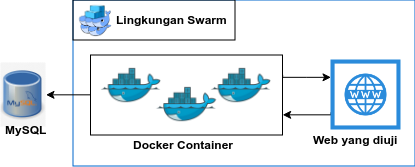
\includegraphics[width=10cm,height=4.5cm]{Images/C-3/puppdesain.png}
    			\caption{Desain pengambil data uji beban}
    			\label{puppdesain}
    		\end{figure}
    	
    	\subsection{Perancangan Service Controller}
    		Komponen ini akan digunakan untuk mengatur segala proses uji beban pada sistem. Pada komponen ini akan terdapat 3 buah sub-komponen yaitu web service, basis data dan task queue atau antrian.
    	
	    	\subsubsection{Desain Web Service}
	    		Web service akan berfungsi sebagai antarmuka pengguna dan sebagai penghubung antara user dengan kontainer. Antarmuka pengguna berfungsi memudahkan user untuk membuat skenario yang akan dikirimkan ke load generator dan kemudian load generator akan melakukan uji beban sesuai dengan skenario yang dikirim user melalui web service. Sedangkan untuk mengatur segala aktivitas user dibutuhkan sebuah controller dan rute yang akan dipasang pada web service. Desain antarmuka pengguna ditunjukkan pada Gambar \ref{mockupweb}.
	    		\begin{figure}[H]
	    			\centering
	    			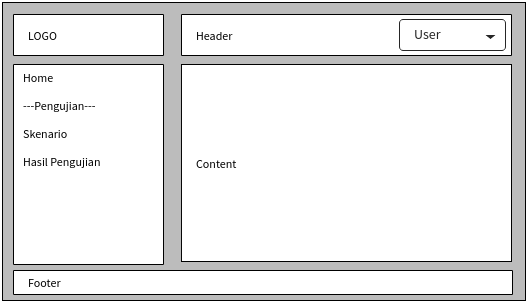
\includegraphics[width=10cm,height=6cm]{Images/C-3/mockupweb.png}
	    			\caption{Desain antarmuka pengguna}
	    			\label{mockupweb}
	    		\end{figure}
	    	
		    	Selain itu, akan dirancang juga fitur-fitur pada web service yang akan digunakan user antara lain:
		    	\begin{enumerate}
		    		\item Menambah dan menghapus skenario.
		    		\item Menentukan jumlah worker pengujian.
		    		\item Melihat performa hasil pengujian.
		    		\item Melihat tangkapan layar tampilan web yang diuji.
		    		\item Melihat console error.
		    		\item Melihat status antrian proses uji. \\
		    	\end{enumerate}
	    		
	   		\subsubsection{Desain Basis Data}
	   			Komponen basis data diperlukan untuk menyimpan data-data yang berkaitan dengan sistem. data yang disimpan adalah data node host swarm, data kontainer, data pengguna, data skenario pengujian, data antrian request, data hasil pengujian, data error console, data rata-rata hasil pengujian. Dari data-data tersebut maka dibutuhkan suatu tabel diantaranya yaitu:
	   			\begin{itemize}
	   				\item Tabel swarms \\
	   					Menyimpan data nohe host yang tergabung di dalam lingkungan swarm.
	   				\item Tabel containers \\
	   					Menyimpan data Docker Container yang telah dipersiapkan.
	   				\item Tabel users \\
	   					Menyimpan data pengguna.
	   				\item Tabel scenarios \\
	   					Menyimpan data skenario pengujian.
	   				\item Tabel queues \\
		   				Menyimpan data antrian request pengujian dari user.
	   				\item Tabel results \\
	   					Menyimpan data hasil pengujian yang dilakukan setiap kontainer.
	   				\item Tabel errors \\
	   					Menyimpan data console error yang ada di browser.
	   				\item Tabel summary results \\
	   					Menyimpan data rata-rata hasil pengujian setiap skenario.
	   			\end{itemize}
	    		
	    	\subsubsection{Desain Penggunaan Task Queue}
	    		Pada service controller akan ada banyak request dari user, setiap request tentu saja akan terdapat proses yang akan berjalan dalam jangka waktu yang cukup lama. Jika proses tersebut berada di dalam fungsi yang dipanggil melalui protokol HTTP, maka akan memberikan umpan balik setelah semua proses yang ada dibaliknya selesai. Hal ini akan membuat user yang melakukan request perlu menunggu dan tidak efisien. Untuk mengatasi hal ini, akan dirancang sebuah komponen antrian atau bisa disebut task queue. Task queue akan membuat antrian untuk setiap request dibelakang layar. Antrian request tersebut akan disimpan pada basis data MySQL.